% Options for packages loaded elsewhere
\PassOptionsToPackage{unicode}{hyperref}
\PassOptionsToPackage{hyphens}{url}
%
\documentclass[
]{article}
\usepackage{amsmath,amssymb}
\usepackage{iftex}
\ifPDFTeX
  \usepackage[T1]{fontenc}
  \usepackage[utf8]{inputenc}
  \usepackage{textcomp} % provide euro and other symbols
\else % if luatex or xetex
  \usepackage{unicode-math} % this also loads fontspec
  \defaultfontfeatures{Scale=MatchLowercase}
  \defaultfontfeatures[\rmfamily]{Ligatures=TeX,Scale=1}
\fi
\usepackage{lmodern}
\ifPDFTeX\else
  % xetex/luatex font selection
\fi
% Use upquote if available, for straight quotes in verbatim environments
\IfFileExists{upquote.sty}{\usepackage{upquote}}{}
\IfFileExists{microtype.sty}{% use microtype if available
  \usepackage[]{microtype}
  \UseMicrotypeSet[protrusion]{basicmath} % disable protrusion for tt fonts
}{}
\makeatletter
\@ifundefined{KOMAClassName}{% if non-KOMA class
  \IfFileExists{parskip.sty}{%
    \usepackage{parskip}
  }{% else
    \setlength{\parindent}{0pt}
    \setlength{\parskip}{6pt plus 2pt minus 1pt}}
}{% if KOMA class
  \KOMAoptions{parskip=half}}
\makeatother
\usepackage{xcolor}
\usepackage[margin=1in]{geometry}
\usepackage{longtable,booktabs,array}
\usepackage{calc} % for calculating minipage widths
% Correct order of tables after \paragraph or \subparagraph
\usepackage{etoolbox}
\makeatletter
\patchcmd\longtable{\par}{\if@noskipsec\mbox{}\fi\par}{}{}
\makeatother
% Allow footnotes in longtable head/foot
\IfFileExists{footnotehyper.sty}{\usepackage{footnotehyper}}{\usepackage{footnote}}
\makesavenoteenv{longtable}
\usepackage{graphicx}
\makeatletter
\def\maxwidth{\ifdim\Gin@nat@width>\linewidth\linewidth\else\Gin@nat@width\fi}
\def\maxheight{\ifdim\Gin@nat@height>\textheight\textheight\else\Gin@nat@height\fi}
\makeatother
% Scale images if necessary, so that they will not overflow the page
% margins by default, and it is still possible to overwrite the defaults
% using explicit options in \includegraphics[width, height, ...]{}
\setkeys{Gin}{width=\maxwidth,height=\maxheight,keepaspectratio}
% Set default figure placement to htbp
\makeatletter
\def\fps@figure{htbp}
\makeatother
\setlength{\emergencystretch}{3em} % prevent overfull lines
\providecommand{\tightlist}{%
  \setlength{\itemsep}{0pt}\setlength{\parskip}{0pt}}
\setcounter{secnumdepth}{5}
\newlength{\cslhangindent}
\setlength{\cslhangindent}{1.5em}
\newlength{\csllabelwidth}
\setlength{\csllabelwidth}{3em}
\newlength{\cslentryspacingunit} % times entry-spacing
\setlength{\cslentryspacingunit}{\parskip}
\newenvironment{CSLReferences}[2] % #1 hanging-ident, #2 entry spacing
 {% don't indent paragraphs
  \setlength{\parindent}{0pt}
  % turn on hanging indent if param 1 is 1
  \ifodd #1
  \let\oldpar\par
  \def\par{\hangindent=\cslhangindent\oldpar}
  \fi
  % set entry spacing
  \setlength{\parskip}{#2\cslentryspacingunit}
 }%
 {}
\usepackage{calc}
\newcommand{\CSLBlock}[1]{#1\hfill\break}
\newcommand{\CSLLeftMargin}[1]{\parbox[t]{\csllabelwidth}{#1}}
\newcommand{\CSLRightInline}[1]{\parbox[t]{\linewidth - \csllabelwidth}{#1}\break}
\newcommand{\CSLIndent}[1]{\hspace{\cslhangindent}#1}
\usepackage{svg}
\usepackage{floatrow}
\usepackage{booktabs}
\usepackage{longtable}
\usepackage{array}
\usepackage{multirow}
\usepackage{wrapfig}
\usepackage{float}
\usepackage{colortbl}
\usepackage{pdflscape}
\usepackage{tabu}
\usepackage{threeparttable}
\usepackage{threeparttablex}
\usepackage[normalem]{ulem}
\usepackage{makecell}
\usepackage{xcolor}
\ifLuaTeX
  \usepackage{selnolig}  % disable illegal ligatures
\fi
\IfFileExists{bookmark.sty}{\usepackage{bookmark}}{\usepackage{hyperref}}
\IfFileExists{xurl.sty}{\usepackage{xurl}}{} % add URL line breaks if available
\urlstyle{same}
\hypersetup{
  pdftitle={Self-absorbed, yet interesting?},
  pdfauthor={Piotr Bystranowski},
  hidelinks,
  pdfcreator={LaTeX via pandoc}}

\title{Self-absorbed, yet interesting?}
\usepackage{etoolbox}
\makeatletter
\providecommand{\subtitle}[1]{% add subtitle to \maketitle
  \apptocmd{\@title}{\par {\large #1 \par}}{}{}
}
\makeatother
\subtitle{A study on general jurisprudence}
\author{Piotr Bystranowski}
\date{2023-12-12}

\begin{document}
\maketitle
\begin{abstract}
Two kinds of critism can be raised against contemporary general jurisprudence -- the part of legal philosophy dealing with the most general and abstract philosophical questions about law. The more fundamental one claims that questions discussed by general jurisprudence might actually not be interesting. The other one, while not denying the overall utility of general jurisprudence, suspects that, as currently practiced, it suffers from self-referentiality and lack of interest in other related philosophical discources. In this article, I attempt to test both propositions empirically, using bibliometric tools. First, employing co-citation analysis, I identify the set of 169 central texts in general jurisprudence within the broader network of 713 core texts in (mostly Anglophone) legal philosophy. This provides ground for the analysis of citation flows, resulting in the following conclusions: General jurisprudence, when compared to other areas of legal philosophy, \emph{is} distinctively self-referential, yet it still appears to spark \emph{some} interest among other scholars, in legal philosophy and elsewhere.
\end{abstract}

{
\setcounter{tocdepth}{2}
\tableofcontents
}
General jurisprudence -- the part of legal philosophy dealing with the most general and abstract questions about law -- is increasingly characterised in terms of stagnation, lack of progress and fixation with decades-long debates. Many have stressed the apparent isolation of this area and, as it often happens, the isolation of a research community can be manifested in two ways: in the community not being interest\emph{ed} in the developments in the outside world as well as in it not being interest\emph{ing} for the outsiders. And so, general jurisprudence has been accused of not being informed or taking inspiration from relevant areas of philosophy, such as metaethics (Plunkett and Shapiro 2017) or not attempting to engage more with philosophical problems arising in specific areas of legal scholarship, while sticking to decades-old debates without noticing that they might have reached a dead end (Hershovitz).

On the other hand, somewhat more fundamentally, some have argued that general jurisprudence is in principle not interesting. One way in which general jurisprudence is not interesting is its putative lack of impact on first-order controversies in specific areas of law (Hershovitz 2014, 1200--1201). Unlike in ethics, where the answer to a question in normative ethics often depends on one's position in metaethics, an analogical dependence is rare in the legal domain\footnote{``Hart and Dworkin may differ with regard to the best account of what's going on when a judge exercises (some kind of) discretion, but it's not at all clear that what you should do as a judge in such cases depends on whether Hart of Dworkin are right'' (Enoch 2019, 82).}. Another way to look at this putative isolation is to draw an analogy with similar yet better analysed research communities. To the extent that general jurisprudence is considered to occupy the centre of legal philosophy, it might parallel the patterns of the core of philosophy: epistemology, metaphysics, philosophy of language. Earlier studies (Kitcher 2011), including ones presenting bibliometric evidence (Chi and Conix 2022; Higgins and Dyschkant 2014), suggested that the core of philosophy, while enjoying much prestige within the discipline, is much less likely to interact with the outside world (scholarly or otherwise) than the seemingly more peripheral areas of philosophy. Philosophy of physics, say, while not being at the centre of philosophy, is more likely to read and be read by scholars from other disciplines than contemporary metaphysics. Should we expect analogical patterns in the case of general jurisprudence?

Following similar studies conducted in other areas of philosophy, here I attempt to assess and analyse the putative isolation of general jurisrpudence using bibliometric tools, primarily: citation analysis. However, to do that in an empirical and rigorous way, one would hope to start with some idea of what the object of study -- general jurisprudence -- is. Some interesting potential definitions have been proposed in the literature\footnote{``\,`general jurisprudence' should refer to the subset of meta-legal inquiry that concerns universal legal thought, talk, and reality, that is, the part of legal thought and talk---and what (if anything) they are distinctively about---that is universal across all social/historical contexts where there is such thought and talk'' (Plunkett and Shapiro 2017, 45);} {[}blablabla{]} but many scholars discussing general jurisprudence doubt any such definition is needed. In this study, I will let the data speak in order to determine if there is a bottom-up way of delineating an are of research that would correspond to what scholars have in mind when they discuss general jurisprudence.

Let me make one important caveat from the start. Whatever evidence based on citation analysis I am going to present, I do not expect all the participants to the debate on the nature and status of general jurisprudence to find it convincing or even relevant. Take scholars who claim that general jurisprudence does not bring valuable arguments to first-order discussions in specific areas of law. Would such a statement be refuted by results showing that legal scholars or more specialized legal philosophers cite general jurisprudence at decent rates? Of course not, scholarly citation patterns depend on many factors, with the actual relevance of the cited work to the citing work being merely one of them\footnote{See the section \emph{Limitations} below for further discussion}. Furthermore, even if a given legal scholar/philosopher \emph{thinks} that general jurisprudence is relevant to their investigations, they might be simply mistaken -- a posssiblity explicitly defended by some of the discussed critics (Enoch 2019, 83 ff.)

\hypertarget{earlier-research}{%
\section{Earlier research}\label{earlier-research}}

Bibliometric tools, such as analysis of citation patterns or coauthorship networks, have traditionally been used in general scientometrics research. Recently, however, they have started to be increasingly used to address questions relevant from the points of view of specific areas of academic research. Take philosophy -- over the last couple of years, citation analysis tools have been used to address problems such as: the partition of philosophy into main areas of research (Noichl 2021); the visibility of philosophy of science in the sciences (Khelfaoui et al. 2021); the relative isolation of some areas of philosophy from non-philosophical literature (Chi and Conix 2022).

To this date, hardly any attempt at using citation analysis to map research communities within legal philosophy or, even much broader, legal scholarship exists. It is so despite the increasing usage of co-authorship (Hayashi 2022), hiring-and-placement (Katz et al. 2011) or acknowledgment (Nunna et al. 2023) networks in sociological analyses of the structure of legal academia and, even more strikingly, the already established centrality of citation networks as a research tool in empirical analyses of case law across jurisdictions (Derlén and Lindholm 2014; Fowler et al. 2007; Hitt 2016; Šadl and Olsen 2017; Siems 2023; Smejkalová 2020). Despite the methodological parallels, none of these studies addressed the issue central to this paper: the measurement of the degree of isolation of a given fragment of legal scholarship.

In this project, I aim to employ co-citation analysis\footnote{While a \emph{citation} refers to a relation in which one article cites another, a \emph{co-citation} is a relation between two articles that have been jointly cited by at least one third article. For one thing, co-citation, unlike citation, is a symmetrical relation.} -- a tool used to measure subject similarity and intellectual connections between pairs of academic texts (Small 1973) -- to identify the core of contemporary philosophy of law (i.e., a set of legal philosophical texts that are most frequently co-cited with each other) and to partition the graph representing this core into areas representing distinct areas of research and/or distinct epistemic communities in philosophy of law as well as to describe the structure of such a graph, in particular -- the position of the community corresponding to general jurisprudence. Completing those tasks, which might be of some independent value, will prepare ground for addressing two main questions. First, to what extent different areas of philosophy of law, especially general jurisprudence, interact with each other. Second, which areas of philosophy of law are visible in academic literature outside this discipline.

\hypertarget{network-construction}{%
\section{Network construction}\label{network-construction}}

As I intended to start this study with situating general jurisprudence within the core of legal philosophy, the necessary first step was to find a way of delineating the set of texts representing legal philosophy. There are three general (and combinable) approaches in bibliometrics to domain delineation: using ready-made classifications of science, classical information-retrieval searches, mapping and clustering (Zitt et al. 2019). The first approach, typically taking advantage of existing categorizations of journals, was not feasible here, for a number of reason. First, which alone would be sufficient, none of the leading journal classification involves a separate category for philosophy of law. Second, even if there were such a classification, I assumed that much of crucial work in legal philosophy is published outside specialist journals (crucially, in books or journals that are not indexed in the leading citation data bases), so such an approach would likely result in a distorted picture of the field. \ldots.

All the citation data used in this project come from \emph{OpenAlex}, an open bibliometric data base (Priem, Piwowar, and Orr 2022). While \emph{OpenAlex} remains less frequently used in research of the kind I conduct here than its proprietary substitutes (such as \emph{Web of Science}) and it presents some important limitations\footnote{See the section \emph{Limitations} below.}, it offers some considerable advantages in the present context. The most important feature is the breadth of its coverage. While any bibliometric analysis of legal philosophy limited to the WoS-indexed journals would present an incomplete if not biased picture, \emph{OpenAlex} covers many non-WoS-indexed journals and books, which, arguably, remain an important venue for work in jurisprudence.

The process of constructing the graph representing the core of legal philosophy, largely inspired by similar work by Truc (2022), proceeded as follows (Figure \ref{fig:flowchart}). The first step was to collect available metadata for all articles published in journals publishing work exclusively or primarily in philosophy of law and legal theory. I set a list of 19 such journals, including 13 published outside the English-speaking countries (in an attempt to construct a more diverse data set and to minimize the bias toward legal scholarship published in English).\footnote{As I will discuss in more detail later, this attempt might have been not entirely successful, due to some shortcomings of the employed data based.} This resulted in a set of over 12.5 thousand papers. As most of those items have not been, according to the employed data base, cited even once, and, thus, were unlikely to play any role in the subsequent analyses, I narrowed down the data set to articles cited at least once, which resulted in a collection of 4,683 items, which I call the `Specialist Journal Collection'.

Then, however, I could not limit the study to the Specialist Journal Collection, for at least two reasons. First, one might argue that the most important articles in legal philosophy are often published outside specialist journals. Philosophers of law tend to publish their work in generalist legal journals (such as student-run U.S. law reviews) on the one hand, and in less specialized philosophy journals (say, in moral or political philosophy), on the other. Furthermore, while in many areas, particularly in the sciences, the relevant scientific output is reducible to journal articles, this is not the case with philosophy of law, where books are still very much focal. Not only many contemporary discussions are based on ideas presented in seminal books published in the 1960s or 70s but also many legal philosophical books published today have a greater impact than most journal articles published in the same time.

For those reasons, I expanded the data set in two further steps. First, I assumed that any text that cites a significant number of items published in specialist journals in legal philosophy is likely a text in legal philosophy itself. Hence, I created a collection of papers that cite at least 6 items from the Specialist Journal Collection. The resulting Citing Collection included 923 additional items. Second, I assumed that many classical works in legal philosophy could still be missing from both collections (as they were neither published in specialist journals, nor did they cite specialist journals). To identify such classical works, I created a collection of texts cited at least 6 times in the combined Specialist Journal and Citing collections, resulting in 1,045 additional items. That collection, however, was clearly over-inclusive, as it covered many pieces that are heavily cited across different fields, thus hardly specific to legal philosophy. This was the case of some notable piece from social sciences (such as classical works in psychology by Haidt or Kahneman and Tversky or in economics by Coase), but also for some focal work in philosophy: Even though it was directly relevant to some discussions in jurisprudence, it could not be reasonably called legal even in the broadest sense (take Quine, JL Austin, or Searle). As such items, by definition, are heavily cited, they were likely to affect the analyses to follow. To remedy this issue, I calculated the ratio of the number of citations coming from the Specialist Journal and Citing collections to the overall number of citations for each of the classics papers. The assumption here was that papers for which a significant proportion of citations comes from the former are likely papers in legal philosophy. However, the choice of the exact threshold involves some important trade-offs. As some important works in legal philosophy are heavily cited also outside this specific area, setting the threshold too high would leave such important items (such as, say, \emph{On the Rule of Law} by Tamanaha) out. Ultimately, I decided that all the items for which the said ratio was below 0.015 were to be excluded. Arbitrary as this choice was, it excluded a few important papers in legal philosophy (e.g., \emph{Substantive and Reflexive Elements in Modern Law} by Teubner), while keeping some work more readily belonging to moral or political philosophy (e.g., \emph{Moral Thinking} by Hare or \emph{Contractualism and utilitarianism} by Scanlon). While the impact of such occasional mismatches on the analyses to follow should not be overstated, it is worth keeping in mind. All in all, the resulting Classics Collection, after exclusions, contained 888 items.

The three collections combined (4,077 items) provided the basis for the co-citation analysis, which used all the citations that any of those texts received, according to the employed data base (171,974 citations in total). The co-citation analysis was conducted using the \texttt{biblionetwork} package in R (Goutsmedt, Claveau, and Truc 2021). The most important parameter set by the researcher while running the cocitation analysis is the weight\footnote{In \texttt{biblionetwork}, the weight is the number of times the two items are cited together divided by the square root of the product of the total number of citations of each item -- a measure similar to the coupling angle value (Sen and Gan (1983))} threshold: Intuitively, the higher the threshold is, the more times two items need to be cited together (other things being equal) to be connected in the resulting co-citation graph. In practical terms, setting a high threshold tends to result in more structured graphs at the expense of lowering the number of items included in the graph (as more items are left unconnected to any other item).

\begin{figure}
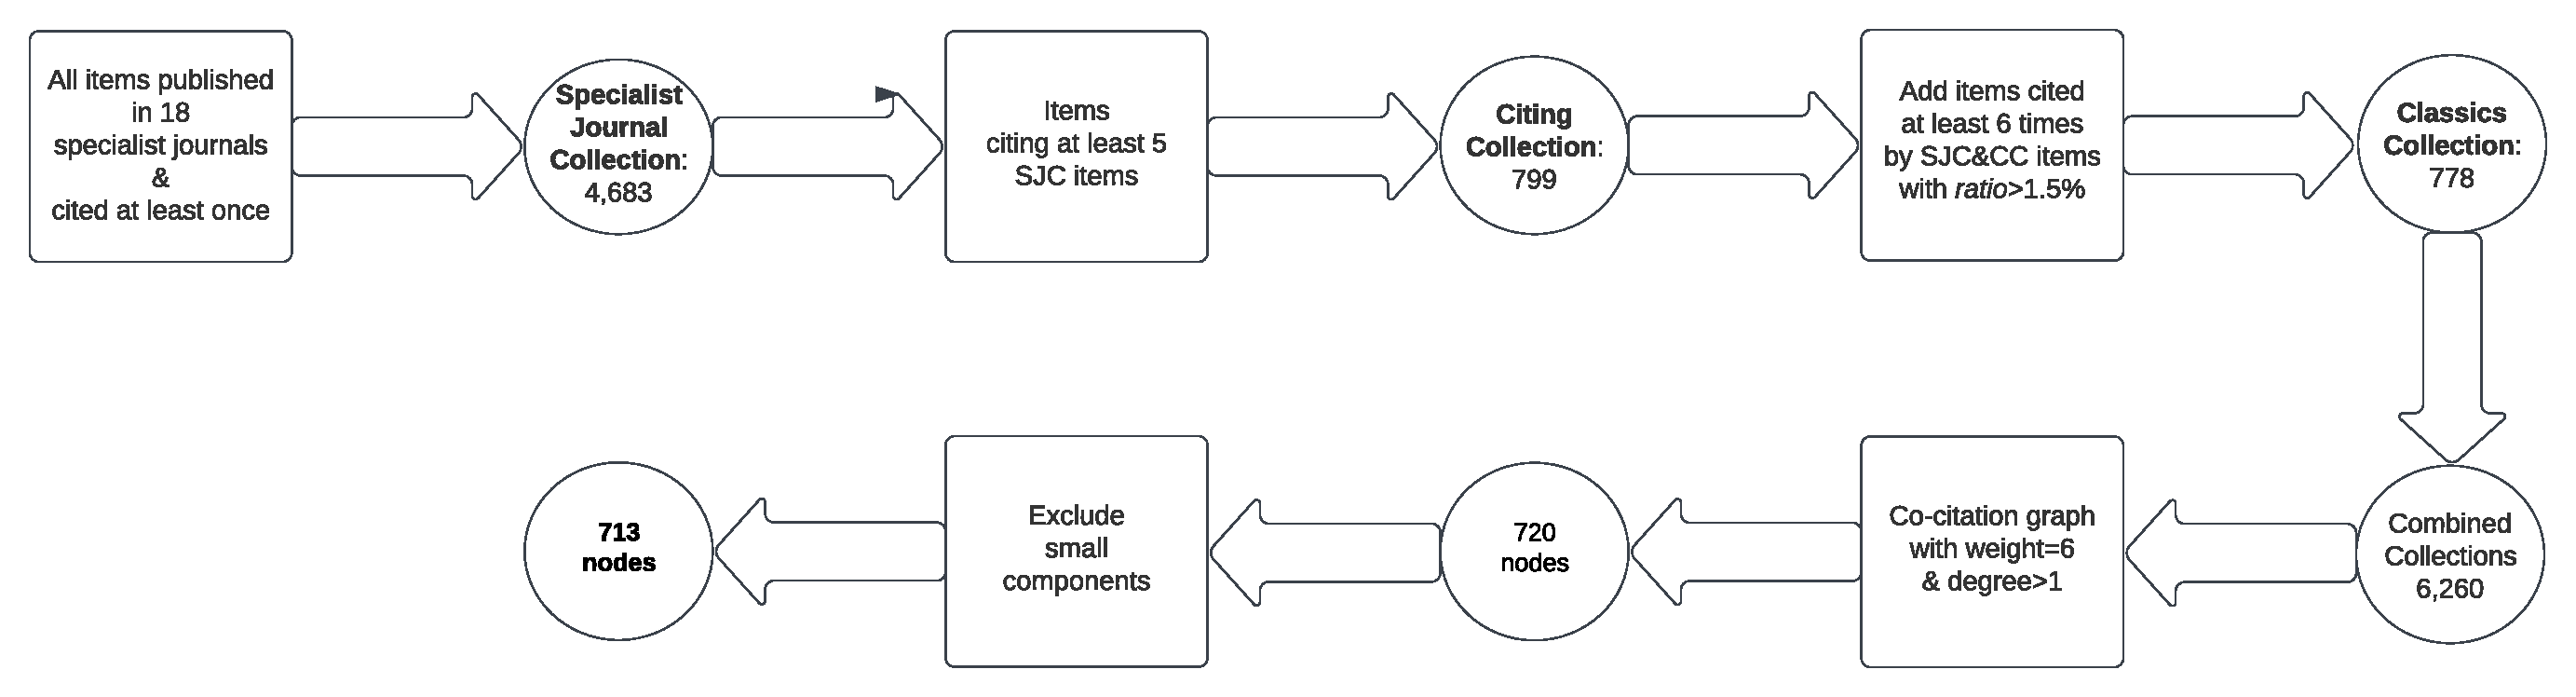
\includegraphics[width=1\linewidth]{flowchart} \caption{The graph construction process}\label{fig:flowchart}
\end{figure}

In the present context, I set the weight threshold to 6. Furthermore, to avoid the inclusion of items that are items connected to just one other item (which might be might be just a result of noise), I included in the graph only items connected to at least two other items. The resulting graph consisted of 720 nodes (representing 720 texts from the combined collections) and three connected components. Two of those components were extremely small (four and three nodes, respectively)\footnote{Both of the small components appered to represent rather niche discussions in the theory of criminal responsibility.} and were discarded. Thus, only the big component of the co-citation graph, consisting of 713 nodes, was retained and will the object of the analyses to follow (Figure \ref{fig:figSvg}.

\hypertarget{network-interpretation}{%
\section{Network interpretation}\label{network-interpretation}}

One of the main analyses to conduct with a connected graph is to identify its distinct \emph{communities}, that is, sets of nodes that are better connected to each other than they are to the rest of the graph. In the case of cocitation networks, such communities might correspond to different areas of research and/or different epistemic communities. Partitioning a graph into communities is conducted using computational algorithms, which are typically probabilistic and dependent on parameters arbitrarily set by the researcher. Here, I used the Louvain algorithm (Blondel et al. 2008) as implemented in Gephi (Bastian, Heymann, and Jacomy 2009) with the default resolution, which resulted in XXX communities. The communities were rather heterogeneous in terms of their size, with a few big communities and many small ones. As the smallest communities would be hard to interpret or to conduct any meaningful analyses, I retained the 19 biggest communities (with at least XXX members) which I was able to interpret, that is, to map onto discrete areas of legal philosophical research.

In this interpretative process, I used two main tools. First, for each community I identified specific texts that were most important for a given community, as measured by eigenvector centrality\footnote{In graph analysis, eigenvector centrality measures what intuitively could be interpreted as the prestige of a given node within the network, where prestige of a given node is determined by being directly linked to other nodes that are prestigious themselves. For more detail, see Section \emph{Centrality} below.}. Second, for each community I identified the set of most characteristic terms from titles and abstracts of texts in a given community. To characteristic terms I used a classical measure used in text analysis, text frequency-inverse document frequency (tf-idf).

\begin{figure}
\includegraphics[width=1\linewidth]{t} \caption{The big component of the cocitation graph. Edge thicknes is proportional to the cocitation weight, as described in footnote 2. Node size is proportional to the eigenvector centrality. Gephi’s Multigravity ForceAtlas 2 was used for layout rendering.}\label{fig:figSvg}
\end{figure}

Let us illustrate the interpretive process by describing in more detail the four And so, the largest community (spanning well over a fifth of the entire graph) can be interpreted as denoting \textbf{\emph{General jurisprudence}}. Two central figures of the twentieth-century Anglophone general jurisprudence\footnote{Throughout the article, I use `\emph{General jurisprudence}' to refer to the specific community (subgraph) detected within the analysed graph and `general jurisprudence' to refer to the actual research area and scholarly community} -- H.L.A. Hart and Ronald Dworkin -- authored five out of 10 most central texts in this community and their surnames feature among the terms most characteristic for the community. Inasmuch contemporary general jurisprudence has been focused around debates surrounding legal positivism, so is the analyzed community. All 10 most central texts are written either by notable advocates of positivism -- Hart, John Austin, Joseph Raz -- or its harshest critics -- Dworkin, Lon Fuller, John Finnis. Furthermore, the terms \emph{positivism} and \emph{positivist} are the two terms most characteristic of the community. The remainder of the set of most characteristic terms deals primarily with exactly those concepts that we would associate with the most abstract reflection on law: \emph{judge}, \emph{theory}, \emph{rule}, \emph{jurisprudence}, \emph{interpretation}.

The next largest community appears to deal with issues at the intersection of legal and political philosophy. Many of the authors of the most central texts are more readily labelled as political, not legal, philosophers (Thomas Nagel, John Rawls). One can, however, still see the legal dimension of this cluster. The most characteristic terms, even though unmistakenly political, largely deal with those concepts that are relevant to law: \emph{legitimacy}, \emph{democratic}, \emph{neutrality}, \emph{global {[}justice{]}}. Some of the most prominent authors still can be reliably interpreted as legal philosophers, think of Jeremy Waldron or A. John Simmons. For these reasons, I labelled the community \textbf{\emph{Law and political theory}}.

The third community, labelled \textbf{\emph{Punishment}}, appears very straightforward to interpret, with all ten central texts dealing with legal punishment and characteristic terms such as \emph{restorative}, \emph{punishment}, \emph{desert}, \emph{retributive}, \emph{censure}, \emph{expressive}. This contrasts with the next community, \textbf{\emph{Responsibility}} -- here, again, the authors of central texts are mostly philosophers not necessarily associated with law. A closer look at their works, however, as well as at the characteristic terms (such as \emph{responsibility}, \emph{ignorance}, \emph{blameworthiness}, \emph{luck}) suffices to understand that the community deals with the theory of responsibility and other related issues at the intersection of law and moral philosophy (such as moral luck, mental states, moral ignorance, the role of free will).

Let me also notice that, for some smaller communities, I could not easily find one label to capture the apparent object of interest of a given cluster. In some cases, a community appeared to be concerned with two or more distinct yet intrinsically linked constructs (e.g., \textbf{\emph{Judicial review and constitutional rights}}, \textbf{\emph{War, killing, self-defence}}), while at other times topics that do not appear necessarily linked were grouped together (e.g., \textbf{\emph{Theories of rights / Contract law}}, \textbf{\emph{Torts / Causation}}).

\hypertarget{network-analysis}{%
\section{Network analysis}\label{network-analysis}}

Some general observations follow from the inspection of this graph. First of all, this study does not bring us much closer to a precise delineation of legal philosophy. As we just saw, some of the analysed communities (such as \emph{Law and political theory} or \emph{Responsibility} feature texts that appear to clearly belong to other areas of practical philosophy. This, however, need not necessarily be interpreted as a shortcoming of this study but rather as evidence of an intense exchange between some areas of philosophy of law and adjacent epistemic communities. What is really striking, then, is that, in contract, we can see many communities in the analyzed grpah that seem distinctly pure in their legal-philosophical profile, and such is the main object of this study, \emph{General jurisprudence}.

Other initial observations about \emph{General jurisprudence} follow. Most strikingly, while the analyzed graph partition provides an otherwise fine-grained picture of the field, \emph{General jurisprudence} is an outlier in terms of its size and, as it is very well-connected, there appears no obvious way of dividing it further. The two smaller communitites that arguably belong to general jurisprudence, labelled \emph{Natural law} and \emph{Non-positivism} , are very tiny and well-connected to \emph{General jurisprudence} (so that their separation from \emph{General jurisprudence} might be interpreted as an accidental artifact of the community-detection algorithm rather than a reflection of a deeper separation in the real world).\footnote{In the context of \emph{Natural law}, a striking observation is that, even though the community indeed appears to bring together most natural law texts present in the graph, some notable texts in the natural law tradition ended up in the \emph{General jurisprudence} cluster, just think of Finnis' \emph{Natural law and natural rights}. {[}something about anti-positivism and dworkin being in GJ{]}} While general jurisprudence is often seen as a field defined by persisting debates and disagreements, it seems that it has not resulted in any kind of division of this area into separate epistemic communities. Notably, even representatives of some heterodox approaches to jurisprudence, such as advocates of the Critical Legal Studies movement, sit solidly in \emph{General jurisprudence} rather than form a community of their own.

All in all, this partition of the graph suggests a notion of general jurisprudence that is wider from that employed by at least some scholars. It certainly covers `Oxford jurisprudence', discussion of normativity, rules, and separation of law and morals, but it also shows that all those issues paradigmatically belonging to general jurisprudence are not easily separated from such areas as legal interpretation..

Roughly the same thing can be said about the entire graph -- its partition is almost exclusively based on objects of interest rather than different perspectives or methodologies. For example, while texts written with the law \& economics framework are present in the graph (most prominently with the \emph{Causation / Torts} community), they do not come even close to forming a community on their own.

\hypertarget{centrality}{%
\subsection{Centrality}\label{centrality}}

One of the main upshots of network analysis is the determination of relative importance, or centrality, of nodes within the structure of a given graph. Numerous mathematical tools have been developed to capture differnt aspects of such centrality, two of which will be employed in this study. \emph{Eigenvector centrality} (Bonacich 1987; Kleinberg 1999) assigns high centrality to nodes who have many high-centrality neighbours. In the context of social networks, eigenvector centrality corresponds to the intuition that an important individual is the one who has many direct links to other important individuals. In the present context, it expresses the idea that an important publication is the one that is often co-cited with other important publications. The other centrality measure used here is \emph{betweenness centrality} computes the proportion of the shortest paths between any pair of nodes in the graph that pass through a given node. For social networks, betweenness centrality highlights the importance of individuals who serve as `bridges' and control the flow of information or other goods between otherwise distant individuals. In the present context, betweenness centrality stresses those publications that might serve as meeting points for otherwise distant areas of legal philosophy.

\begin{table}[!h]

\caption{\label{tab:eigenpaper}10 texts with the highest eigenvector centrality.}
\centering
\begin{tabular}[t]{>{\raggedright\arraybackslash}p{3cm}>{\raggedright\arraybackslash}p{5cm}>{\raggedleft\arraybackslash}p{1.5cm}>{\raggedleft\arraybackslash}p{1.5cm}>{\raggedright\arraybackslash}p{5cm}}
\toprule
First author & Title & Eigen- vector centrality & Between- ness centrality & cluster\_label\\
\midrule
\cellcolor{gray!6}{HLA Hart} & \cellcolor{gray!6}{The Concept of Law} & \cellcolor{gray!6}{1.00} & \cellcolor{gray!6}{80561} & \cellcolor{gray!6}{General jurisprudence}\\
Jules L. Coleman & Taking Rights Seriously & 0.83 & 26121 & General jurisprudence\\
\cellcolor{gray!6}{Ronald Dworkin} & \cellcolor{gray!6}{Law's Empire} & \cellcolor{gray!6}{0.83} & \cellcolor{gray!6}{5899} & \cellcolor{gray!6}{General jurisprudence}\\
H. L. A. Hart & Positivism and the Separation of Law and Morals & 0.76 & 22026 & General jurisprudence\\
\cellcolor{gray!6}{Joseph Raz} & \cellcolor{gray!6}{The Morality of Freedom} & \cellcolor{gray!6}{0.74} & \cellcolor{gray!6}{47557} & \cellcolor{gray!6}{General jurisprudence}\\
\addlinespace
John Finnis & Natural Law and Natural Rights. & 0.68 & 6014 & General jurisprudence\\
\cellcolor{gray!6}{Joseph Raz} & \cellcolor{gray!6}{The authority of lawEssays on law and morality} & \cellcolor{gray!6}{0.65} & \cellcolor{gray!6}{4136} & \cellcolor{gray!6}{General jurisprudence}\\
RONALD DWORKIN & A Matter of Principle & 0.63 & 2242 & General jurisprudence\\
\cellcolor{gray!6}{Lon L. Fuller} & \cellcolor{gray!6}{Positivism and Fidelity to Law: A Reply to Professor Hart} & \cellcolor{gray!6}{0.62} & \cellcolor{gray!6}{411} & \cellcolor{gray!6}{General jurisprudence}\\
Jeremy Waldron & Law and Disagreement & 0.58 & 10909 & Judicial review and constitutional rights\\
\bottomrule
\end{tabular}
\end{table}

Table \ref{tab:eigenpaper} presents 10 texts with the highest eigenvector centrality and is overwhelmingly dominated by texts belonging to \emph{General jurisprudence}. Things are slightly more complicated when we move to betweenness centrality, in which case the list of 10 central texts (Table \ref{tab:betpaper}) is dominated by \emph{General jurisprudence} to a much lower degree. This pattern allows for a speculation that, at least for some publications in \emph{General jurisprudence} are high-prestige mostly because they are often co-cited with other high-prestige publications in \emph{General jurisprudence} rather than because of their links to other communities. Nevertheless, when we look at both measures of centrality averaged across communities (Table \ref{tab:centcomm}), we can see \emph{General jurisprudence} exceling at both, although with a visibly smaller lead over the other communities in the case of betweenness centrality.

\begin{table}[!h]

\caption{\label{tab:betpaper}10 texts with the highest betweenness centrality.}
\centering
\begin{tabular}[t]{>{\raggedright\arraybackslash}p{3cm}>{\raggedright\arraybackslash}p{5cm}>{\raggedleft\arraybackslash}p{1.5cm}>{\raggedleft\arraybackslash}p{1.5cm}>{\raggedright\arraybackslash}p{5cm}}
\toprule
First author & Title & Eigen- vector centrality & Between- ness centrality & cluster\_label\\
\midrule
\cellcolor{gray!6}{HLA Hart} & \cellcolor{gray!6}{The Concept of Law} & \cellcolor{gray!6}{1.00} & \cellcolor{gray!6}{80561} & \cellcolor{gray!6}{General jurisprudence}\\
John Rawls & Two Concepts of Rules & 0.41 & 49278 & Punishment\\
\cellcolor{gray!6}{Joseph Raz} & \cellcolor{gray!6}{The Morality of Freedom} & \cellcolor{gray!6}{0.74} & \cellcolor{gray!6}{47557} & \cellcolor{gray!6}{General jurisprudence}\\
John Martin Fischer & Responsibility and Control & 0.16 & 41161 & Responsibility\\
\cellcolor{gray!6}{Guido Calabresi} & \cellcolor{gray!6}{Property Rules, Liability Rules, and Inalienability: One View of the Cathedral} & \cellcolor{gray!6}{0.29} & \cellcolor{gray!6}{28977} & \cellcolor{gray!6}{Torts / causation}\\
\addlinespace
Thomas Nagel & The Problem of Global Justice & 0.27 & 26757 & Law and political theory\\
\cellcolor{gray!6}{Wesley Newcomb Hohfeld} & \cellcolor{gray!6}{Fundamental Legal Conceptions as Applied in Judicial Reasoning} & \cellcolor{gray!6}{0.49} & \cellcolor{gray!6}{26609} & \cellcolor{gray!6}{Theory of rights / Contract law}\\
Jules L. Coleman & Taking Rights Seriously & 0.83 & 26121 & General jurisprudence\\
\cellcolor{gray!6}{H. L. A. Hart} & \cellcolor{gray!6}{Causation in the Law} & \cellcolor{gray!6}{0.26} & \cellcolor{gray!6}{22989} & \cellcolor{gray!6}{Torts / causation}\\
H. L. A. Hart & Positivism and the Separation of Law and Morals & 0.76 & 22026 & General jurisprudence\\
\bottomrule
\end{tabular}
\end{table}
\begin{table}[!h]

\caption{\label{tab:centcomm}10 communities with the highest average eigenvector centrality.}
\centering
\begin{tabular}[t]{>{\raggedright\arraybackslash}p{3cm}>{\raggedleft\arraybackslash}p{1.5cm}>{\raggedleft\arraybackslash}p{1.5cm}>{\raggedleft\arraybackslash}p{1.5cm}>{\raggedleft\arraybackslash}p{1.5cm}}
\toprule
cluster\_label & N & year & Eigen- vector centrality & Between- ness centrality\\
\midrule
\cellcolor{gray!6}{General jurisprudence} & \cellcolor{gray!6}{169} & \cellcolor{gray!6}{1990} & \cellcolor{gray!6}{0.17} & \cellcolor{gray!6}{1495.91}\\
Judicial review and constitutional rights & 52 & 2001 & 0.11 & 410.15\\
\cellcolor{gray!6}{Theory of rights / Contract law} & \cellcolor{gray!6}{41} & \cellcolor{gray!6}{1987} & \cellcolor{gray!6}{0.07} & \cellcolor{gray!6}{1173.80}\\
Law and political theory & 83 & 1998 & 0.06 & 707.10\\
\cellcolor{gray!6}{Non-positivism (Alexy \& Radbruch)} & \cellcolor{gray!6}{13} & \cellcolor{gray!6}{2003} & \cellcolor{gray!6}{0.05} & \cellcolor{gray!6}{218.38}\\
\addlinespace
Torts / causation & 46 & 1985 & 0.05 & 1356.22\\
\cellcolor{gray!6}{Legal reasoning} & \cellcolor{gray!6}{27} & \cellcolor{gray!6}{1986} & \cellcolor{gray!6}{0.04} & \cellcolor{gray!6}{288.15}\\
Punishment & 66 & 1990 & 0.04 & 1344.86\\
\cellcolor{gray!6}{International law} & \cellcolor{gray!6}{22} & \cellcolor{gray!6}{2001} & \cellcolor{gray!6}{0.03} & \cellcolor{gray!6}{245.23}\\
Natural law & 14 & 1995 & 0.03 & 202.79\\
\bottomrule
\end{tabular}
\end{table}

\hypertarget{centrality-vs.-age-and-type-of-publication}{%
\subsubsection{Centrality vs.~age and type of publication}\label{centrality-vs.-age-and-type-of-publication}}

A critic of general jurisprudence might argue that the centrality of the corresponding community, described above, is just an effect of the centrality of a few old books, written by Hart, Fuller, Dworkin, Raz and others, rather than a reflection of the importance of any contemporary discussions in this area. If this assumption is correct and, indeed, characteristic of this community, we should be able to observe that older items and books are associated with a relatively larger eigenvector centrality within \emph{General jurisprudence} than elsewhere. Hence, I fit a number of linear models predicting the eigenvector centrality of nodes (Table \ref{tab:anova}). Adding the interaction between Community (i.e., whether a given node belongs to \emph{General jurisprudence}) and publication\_year improves the model's fit. Figure \ref{fig:inter1} depicts the details of this significant interaction: While we observe a negative effect of time across the board (i.e., newer texts enjoy relatively smaller centrality), this negative trend is much more pronounced for \emph{General jurisprudence}. Consistently with the critics' position, older texts are distinctively central within this community.

Similarly, adding the interaction between Community and Type of publication (i.e., whether a given text is a book) significantly improves the model's fit. Again, while we observe a general trend across communities (i.e., a slightly bigger centrality of books), this trend is strikingly larger for \emph{General jurisprudence} (Figure \ref{fig:inter2}), consistently with the critics' predictions.

\begin{table}[!h]

\caption{\label{tab:anova}Analysis of variance (type II) of the model predicting eigenvector centrality}
\centering
\fontsize{8}{10}\selectfont
\begin{tabular}[t]{lrrrl}
\toprule
term & sumsq & df & F statistic & p value\\
\midrule
\cellcolor{gray!6}{publication\_year} & \cellcolor{gray!6}{0.48} & \cellcolor{gray!6}{1} & \cellcolor{gray!6}{46.32} & \cellcolor{gray!6}{<.001}\\
Community & 1.49 & 2 & 72.13 & <.001\\
\cellcolor{gray!6}{`Type of publication`} & \cellcolor{gray!6}{0.51} & \cellcolor{gray!6}{2} & \cellcolor{gray!6}{24.78} & \cellcolor{gray!6}{<.001}\\
publication\_year:Community & 0.12 & 1 & 11.38 & <.001\\
\cellcolor{gray!6}{publication\_year:`Type of publication`} & \cellcolor{gray!6}{0.00} & \cellcolor{gray!6}{1} & \cellcolor{gray!6}{0.08} & \cellcolor{gray!6}{0.779}\\
\addlinespace
Community:`Type of publication` & 0.17 & 1 & 16.76 & <.001\\
\cellcolor{gray!6}{publication\_year:Community:`Type of publication`} & \cellcolor{gray!6}{0.00} & \cellcolor{gray!6}{1} & \cellcolor{gray!6}{0.06} & \cellcolor{gray!6}{0.801}\\
Residuals & 6.92 & 670 & NA & NA\\
\bottomrule
\end{tabular}
\end{table}

\begin{figure}
\centering
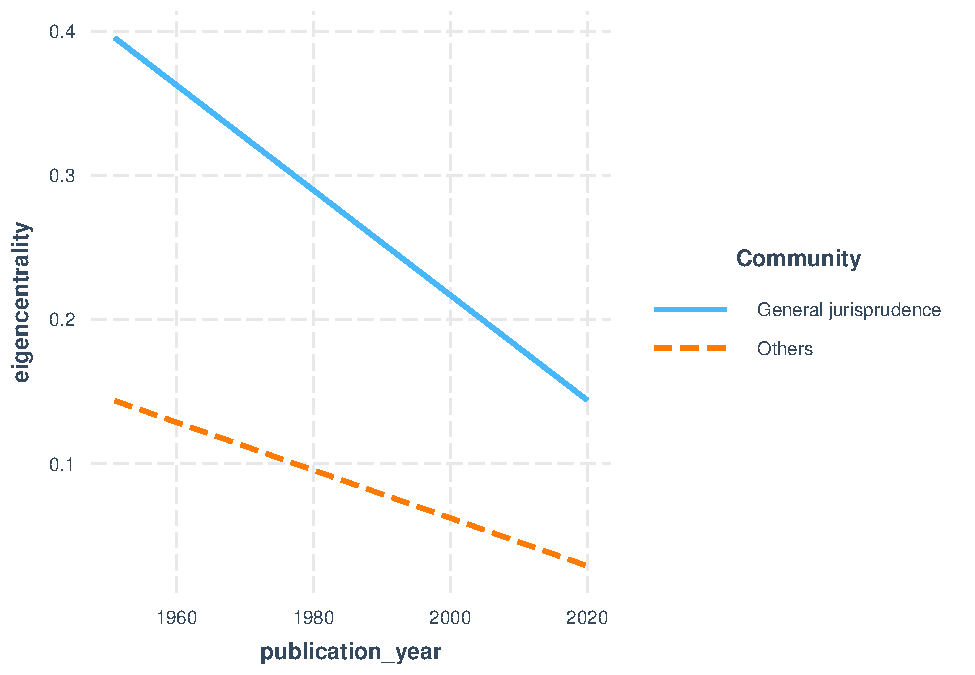
\includegraphics{paper_files/figure-latex/inter1-1.pdf}
\caption{\label{fig:inter1}Interaction between Publication year and Community in the model predciting eigenvector centrality}
\end{figure}

\begin{figure}
\centering
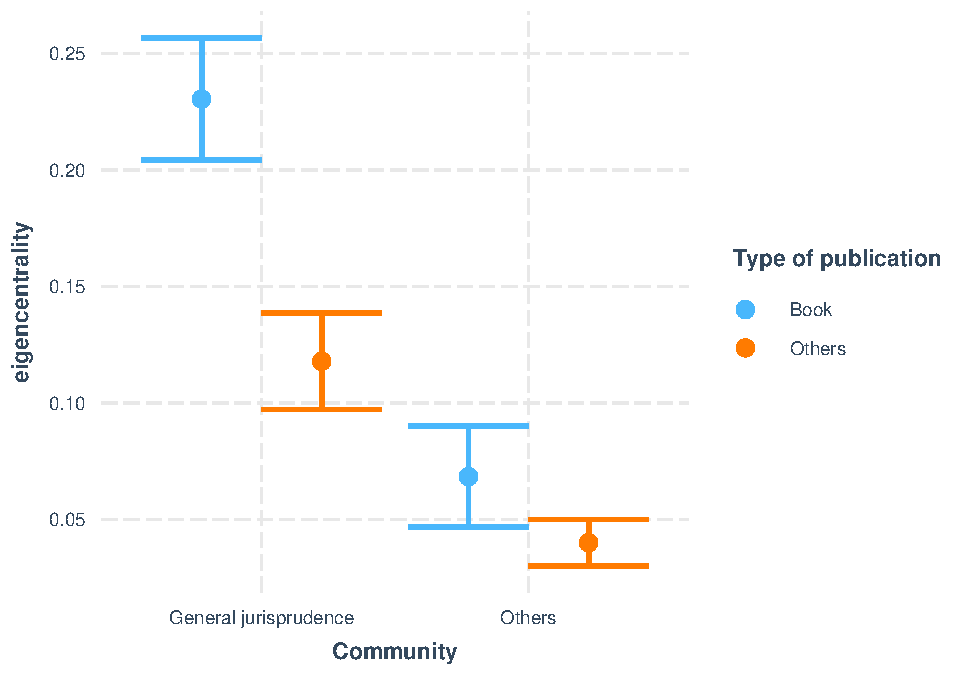
\includegraphics{paper_files/figure-latex/inter2-1.pdf}
\caption{\label{fig:inter2}Interaction between Type of publication and Community in the model predciting eigenvector centrality}
\end{figure}

\hypertarget{citation-flows}{%
\section{Citation flows}\label{citation-flows}}

So far, I have made some observations about the structure of the graph of legal philosophy and the community of \emph{General jurisprudence}, including the centrality of the latter within the graph. To directly address the questions with which this study started, regarding the level engagement of general jurisprudence with other scholarly areas, I will use primarily the tools of citation flow analysis. Notice that co-citation analysis, on which I have been building this study so far, does not measure any direct engagement between texts -- if two texts are connected in a co-citation graph, it means only that they are cited together by other texts and not necessarily that one of them cites the other. Citation analysis, to which I move now, is supposed to measure exactly such a direct engagement of one text with another. I will proceed in two steps. In the first one, I will analyse the flows \emph{within} the graph, to check the extent the various communities identified within the core of legal philosophy borrow ideas from each other. In the second step, I will analyse the extent to which those communities are cited by various research disciplines outside the core of legal philosophy, as identified in this study.

\hypertarget{citations-within-the-graph}{%
\subsection{Citations within the graph}\label{citations-within-the-graph}}

Table \ref{tab:meanCited} presents the mean number of citations that go to a given community from other communities in the analyzed graph (i.e., the total number of such citations divided by the number of texts in a given communities) as well as the ratio of that number to the total number of in-graph citations from a given community (i.e., including both those to other communities and to the community itself). \emph{General jurisprudence} features among the communities with highest ratio, with over a half of all incoming within-graph citations coming from other communities. Furthermore, the average number of incoming within-graph outside-community citations for \emph{General jurisprudence} (1.06) is the third largest\footnote{It is also worth noting that the two communities with a larger value of this statistic are an order of magnitude smaller than \emph{General jurisrpudence}}. Both observation imply that a fair share of interest in general jurisprudence comes from other areas of legal philosophy.

Table \ref{tab:meanCiting}, in contrast, presents the mean number of citation \emph{from} a given community \emph{to} other communities and the ratio of that number to the total number of outgoing in-graph citations from a given community. If we order the list by this ratio, this time we find \emph{General jurisprudence} close to the bottom. Only 16\% of in-graph references of \emph{General jurisprudence} go to other communities. The mean count of such references for \emph{General jurisprudence} (0.71) is the third-lowest. General jurisprudence appears distinctively \emph{uninterested} in other areas of legal philosophy.

We can further corroborate both sets of observations by subtracting the mean number of outgoing citations from the mean number of incoming citations for each community (Table \ref{tab:net}), thus obtaining a \emph{net} citation flow for each community. The number for \emph{General jurisprudence} is positive, again illustrating the thesis that, within legal philosophy, others cite general jurisprudence much more than general jurisprudence cites others.

\begin{table}[!h]

\caption{\label{tab:meanCited}Communities ordered by the ratio of the mean number of citations from other communities in the graph to the mean total number of citations to works from the graph}
\centering
\fontsize{8}{10}\selectfont
\begin{tabular}[t]{>{\raggedright\arraybackslash}p{3cm}>{\raggedleft\arraybackslash}p{2cm}>{\raggedleft\arraybackslash}p{2cm}>{\raggedleft\arraybackslash}p{2cm}}
\toprule
Community & Mean \# of citations from other communities & Mean \# of citations from the graph & Ratio\\
\midrule
\cellcolor{gray!6}{Justifications and excuses} & \cellcolor{gray!6}{1.74} & \cellcolor{gray!6}{1.95} & \cellcolor{gray!6}{0.89}\\
Theory of rights / Contract law & 1.06 & 1.63 & 0.65\\
\cellcolor{gray!6}{General jurisprudence} & \cellcolor{gray!6}{1.14} & \cellcolor{gray!6}{2.06} & \cellcolor{gray!6}{0.55}\\
Law and political theory & 0.75 & 1.39 & 0.54\\
\cellcolor{gray!6}{War and killing} & \cellcolor{gray!6}{1.21} & \cellcolor{gray!6}{2.26} & \cellcolor{gray!6}{0.53}\\
\addlinespace
Risk and prevention in criminal law & 0.75 & 1.50 & 0.50\\
\cellcolor{gray!6}{Consent} & \cellcolor{gray!6}{0.43} & \cellcolor{gray!6}{1.71} & \cellcolor{gray!6}{0.25}\\
Non-positivism (Alexy \& Radbruch) & 0.43 & 1.71 & 0.25\\
\cellcolor{gray!6}{Torts / causation} & \cellcolor{gray!6}{0.37} & \cellcolor{gray!6}{1.57} & \cellcolor{gray!6}{0.24}\\
Legal reasoning & 0.44 & 1.88 & 0.23\\
\addlinespace
\cellcolor{gray!6}{International law} & \cellcolor{gray!6}{0.43} & \cellcolor{gray!6}{1.93} & \cellcolor{gray!6}{0.22}\\
Responsibility & 0.44 & 2.22 & 0.20\\
\cellcolor{gray!6}{Evidence and proof} & \cellcolor{gray!6}{0.22} & \cellcolor{gray!6}{1.33} & \cellcolor{gray!6}{0.17}\\
Judicial review and constitutional rights & 0.25 & 1.43 & 0.17\\
\cellcolor{gray!6}{Punishment} & \cellcolor{gray!6}{0.38} & \cellcolor{gray!6}{2.72} & \cellcolor{gray!6}{0.14}\\
\addlinespace
Hate speech & 0.00 & 1.57 & 0.00\\
\cellcolor{gray!6}{Natural law} & \cellcolor{gray!6}{0.00} & \cellcolor{gray!6}{1.00} & \cellcolor{gray!6}{0.00}\\
\bottomrule
\end{tabular}
\end{table}

\begin{table}[!h]

\caption{\label{tab:meanCiting}Communities ordered by the ratio of the mean number of citations from other communities in the graph to the mean total number of citations from works from the graph}
\centering
\fontsize{10}{12}\selectfont
\begin{tabular}[t]{>{\raggedright\arraybackslash}p{3cm}>{\raggedleft\arraybackslash}p{2cm}>{\raggedleft\arraybackslash}p{2cm}>{\raggedleft\arraybackslash}p{2cm}}
\toprule
Community & Mean \# of citations from other communities & Mean \# of citations from within the graph & Ratio\\
\midrule
\cellcolor{gray!6}{Non-positivism (Alexy \& Radbruch)} & \cellcolor{gray!6}{7.00} & \cellcolor{gray!6}{8.80} & \cellcolor{gray!6}{0.80}\\
Justifications and excuses & 1.17 & 1.83 & 0.64\\
\cellcolor{gray!6}{Risk and prevention in criminal law} & \cellcolor{gray!6}{2.00} & \cellcolor{gray!6}{3.50} & \cellcolor{gray!6}{0.57}\\
Law and political theory & 1.27 & 2.32 & 0.55\\
\cellcolor{gray!6}{Natural law} & \cellcolor{gray!6}{0.67} & \cellcolor{gray!6}{1.33} & \cellcolor{gray!6}{0.50}\\
\addlinespace
Judicial review and constitutional rights & 5.17 & 10.67 & 0.48\\
\cellcolor{gray!6}{Punishment} & \cellcolor{gray!6}{3.32} & \cellcolor{gray!6}{8.26} & \cellcolor{gray!6}{0.40}\\
Responsibility & 2.00 & 5.84 & 0.34\\
\cellcolor{gray!6}{Torts / causation} & \cellcolor{gray!6}{4.00} & \cellcolor{gray!6}{12.40} & \cellcolor{gray!6}{0.32}\\
Hate speech & 2.50 & 8.00 & 0.31\\
\addlinespace
\cellcolor{gray!6}{Legal reasoning} & \cellcolor{gray!6}{1.00} & \cellcolor{gray!6}{3.30} & \cellcolor{gray!6}{0.30}\\
Evidence and proof & 0.80 & 2.80 & 0.29\\
\cellcolor{gray!6}{International law} & \cellcolor{gray!6}{1.17} & \cellcolor{gray!6}{4.67} & \cellcolor{gray!6}{0.25}\\
Theory of rights / Contract law & 0.60 & 2.80 & 0.21\\
\cellcolor{gray!6}{War and killing} & \cellcolor{gray!6}{0.44} & \cellcolor{gray!6}{2.67} & \cellcolor{gray!6}{0.17}\\
\addlinespace
General jurisprudence & 0.71 & 4.43 & 0.16\\
\cellcolor{gray!6}{Consent} & \cellcolor{gray!6}{0.00} & \cellcolor{gray!6}{2.25} & \cellcolor{gray!6}{0.00}\\
\bottomrule
\end{tabular}
\end{table}

\begin{table}[!h]

\caption{\label{tab:netCits}Communities ordered by the difference between the mean number of citations from other communities and the mean number of citations to other communities}
\centering
\fontsize{8}{10}\selectfont
\begin{tabular}[t]{>{\raggedright\arraybackslash}p{3cm}>{\raggedleft\arraybackslash}p{2cm}>{\raggedleft\arraybackslash}p{2cm}>{\raggedleft\arraybackslash}p{2cm}}
\toprule
Community & Mean \# of citations to other communities & Mean \# of citations from other communities & Difference\\
\midrule
\cellcolor{gray!6}{War and killing} & \cellcolor{gray!6}{0.44} & \cellcolor{gray!6}{1.21} & \cellcolor{gray!6}{0.77}\\
Justifications and excuses & 1.17 & 1.74 & 0.57\\
\cellcolor{gray!6}{Theory of rights / Contract law} & \cellcolor{gray!6}{0.60} & \cellcolor{gray!6}{1.06} & \cellcolor{gray!6}{0.46}\\
Consent & 0.00 & 0.43 & 0.43\\
\cellcolor{gray!6}{General jurisprudence} & \cellcolor{gray!6}{0.71} & \cellcolor{gray!6}{1.14} & \cellcolor{gray!6}{0.43}\\
\addlinespace
Law and political theory & 1.27 & 0.75 & -0.52\\
\cellcolor{gray!6}{Legal reasoning} & \cellcolor{gray!6}{1.00} & \cellcolor{gray!6}{0.44} & \cellcolor{gray!6}{-0.56}\\
Evidence and proof & 0.80 & 0.22 & -0.58\\
\cellcolor{gray!6}{Natural law} & \cellcolor{gray!6}{0.67} & \cellcolor{gray!6}{0.00} & \cellcolor{gray!6}{-0.67}\\
International law & 1.17 & 0.43 & -0.74\\
\addlinespace
\cellcolor{gray!6}{Risk and prevention in criminal law} & \cellcolor{gray!6}{2.00} & \cellcolor{gray!6}{0.75} & \cellcolor{gray!6}{-1.25}\\
Responsibility & 2.00 & 0.44 & -1.56\\
\cellcolor{gray!6}{Hate speech} & \cellcolor{gray!6}{2.50} & \cellcolor{gray!6}{0.00} & \cellcolor{gray!6}{-2.50}\\
Punishment & 3.32 & 0.38 & -2.94\\
\cellcolor{gray!6}{Torts / causation} & \cellcolor{gray!6}{4.00} & \cellcolor{gray!6}{0.37} & \cellcolor{gray!6}{-3.63}\\
\addlinespace
Judicial review and constitutional rights & 5.17 & 0.25 & -4.92\\
\cellcolor{gray!6}{Non-positivism (Alexy \& Radbruch)} & \cellcolor{gray!6}{7.00} & \cellcolor{gray!6}{0.43} & \cellcolor{gray!6}{-6.57}\\
\bottomrule
\end{tabular}
\end{table}

\hypertarget{citations-from-or-to-outside-the-graph}{%
\subsection{Citations from or to outside the graph}\label{citations-from-or-to-outside-the-graph}}

In the second part of the citation analysis, I analysed the set of all incoming citations to works belonging to the analyzed graph for which the citation source could be matched with the National Science Foundation three-level classification of journals into academic disciplines\footnote{The NSF classification is frequently employed in similar studies. One of its advantages over the competitors is its disjointness, that is, assigning each journal to just one category on each of the three nested levels. In the present context, its shortcoming is the fact that its coverage is limited to the Web of Science-indexed journals, which excludes citations from non-indexed journals (which are numerous in law and philosophy) and from books. I used the original classification with 9 journals manually reclassified (all of them were philosophy journals, such as \emph{Ethics}, \emph{Synthese}, or \emph{Philosophy \& Public Affairs}, originally classified to other disciplines). To increase legibility, I used just 7 categories from the lowest level (Law, Philosophy, Political Science and Public Administration, Economics, Computers, Management, Criminology), one category from the highest level -- Natural Science and Engineering (NSE; without Computers), and all the residual categories from the medium level}. Table @ref(tab:med\_esp) presents the median number of citations from NSF categories to articles in a given community. As could be expected, a typical article belonging to \emph{General jurisprudence} is likely to be noticed in Law and Philosophy. However, the null median numbers of citations from other analyzed NSF categories (aside from Political Science and Public Administration) indicates a lack of interest in general jurisprudence from other fields.\footnote{A potential alternative explanation of this pattern is the large size and resulting heterogeneity of \emph{General jurisprudence}. Small, specialized communities are likely to be consistently cited by scholars from a specific area outside law and philosophy (see, e.g., Criminology citing \emph{Risk and prevention} and Psychology or Health citing \emph{Consent}), which then can be observed on the level of medians. This is less likely to happen with a large, less specialized communities, as \emph{General jurisprudence}.} A closer look at the table, though, indicates that even the patterns of citations from Law and Philosophy to \emph{General jurisprudence} are more complicated. The median number of citations from Philosophy (2) puts \emph{General jurisprudence} only on the 11th place among 17 communities, suggesting a relatively low level of interest from philosophers. The same statistic regarding citations from Law (4) puts it on the 5th place, thus indicating a relatively high level of interest from legal scholars. Consistently with these results, the ratio\footnote{I do not compare the median values across categories, as, due to a potentially unequal coverage of disciplines by the NSF classification (say, a better coverage of Philosophy than Law), such comparisons might be unreliable. Comparing \emph{ratios}, however, is meaningful and not affected by this risk.} of the median number of citations from Law to the median number of citations from Philosophy (2) puts \emph{General jurisprudence} on the 4th place, which shows a relative overrepresentation of Law in the readership.

What I said in the previous paragraph suggests that \emph{General jurisprudence} is characteristically frequently cited by Law. This is right, yet \emph{General jurisprudence} comes only fifth in terms the median number of citations from Law and when we compare its value of this statistic (4) to the leaders (\emph{International law} -- 10; \emph{Judicial review and constitutional rights} -- 8; \emph{Theory of rights / Contract law} -- 6), we see a significant gap. Overall, general jurisprudence seems to be read by legal scholars, yet it might be far from the most interesting area of legal philosophy to legal scholars.

Recall my earlier analyses addressing the question of whether the interest in general jurisprudence if focused on a bunch of older books rather than more recent discussions. In the present context, if that assumption is right, we will expect citations to \emph{General jurisprudence} to target older texts than citations to other communities. To check it, I calculated the \emph{age} of all external citations by subtracting the publication year of the cited document from the publication year of the citing document\footnote{To limit the effect of citations of extreme ages (many of which appear a result of database errors), I included citations whose age was between 0 and 100 years.}. In this sense, the citations to \emph{General jurisprudence} are indeed older (\(M =\) 27.41 years) than citations to other communities (\(M =\) 20.65 years; \(t(\)\ensuremath{3.993615\times 10^{4}}\()=\) 52.42, \(p < .001\)). This general observation holds true for citations coming from journals classified as Law (\(M_{GJ} =\) 25.66 years; \(M_{nonGJ} =\) 19.79 years; \$t(\(2249.12\))=\$ 8.6, \(p < .001\)) and Philosophy (\(M_{GJ} =\) 19.2 years; \(M_{nonGJ} =\) 18.04 years; \$t(\(1187.89\))=\$ 2.41, \$p = \$ 0.016).

Moving to the final citation analysis, let us take a look at the flow of citations \emph{from} the graph to documents outside the graph (Table \ref{tab:medianRef}). A typical text belonging to \emph{General jurisprudence} cites one article from Philosophy and one article from Law (and no articles from other categories). In terms of the number of citations, it gives \emph{General jurisprudence} the 10th place (along four other communities) for Philosophy and the 9th place (along three other communities) for Law. Just like for incoming citations, the average age of citation outgoing from \emph{General jurisprudence} (\(M =\) 16.84 years) is larger than that of other communities (\(M =\) 14.27 years; \$t(\(485\))=\$ 3.28, \(p =\) 0.001). This general observation holds true for citations to journals classified as Law (\(M_{GJ} =\) 23.37 years; \(M_{nonGJ} =\) 18.15 years; \$t(\(76.79\))=\$ 2.14, \(p =\) 0.036), while the same observed difference for Philosophy is not statistically significant (\(M_{GJ} =\) 17.53 years; \(M_{nonGJ} =\) 15.21 years; \$t(\(120.91\))=\$ 1.58, \$p = \$ 0.12). To sum up, documents belonging to \emph{General jurisprudence} cite rather few sources from outside the core of legal philosophy and the sources they do cite tend to be older -- both observations are consistent with the thesis of the particular self-referentiality of general jurisprudence.

\begin{table}[!h]

\caption{\label{tab:medianRef}Median number of citations to a given discipline from an article in a given community}
\centering
\fontsize{7}{9}\selectfont
\begin{tabular}[t]{>{\raggedright\arraybackslash}p{2cm}>{\raggedleft\arraybackslash}p{1.5cm}>{\raggedleft\arraybackslash}p{1.5cm}>{\raggedleft\arraybackslash}p{1.5cm}>{\raggedleft\arraybackslash}p{1.5cm}>{\raggedleft\arraybackslash}p{1.5cm}>{\raggedleft\arraybackslash}p{1.5cm}}
\toprule
Community & Philosophy & Law & Other Social Sciences & Political Science and Public Administration & Criminology & Computers\\
\midrule
\cellcolor{gray!6}{General jurisprudence} & \cellcolor{gray!6}{1.0} & \cellcolor{gray!6}{1} & \cellcolor{gray!6}{0.0} & \cellcolor{gray!6}{0} & \cellcolor{gray!6}{0} & \cellcolor{gray!6}{0}\\
Law and political theory & 2.0 & 0 & 0.0 & 0 & 0 & 0\\
\cellcolor{gray!6}{Punishment} & \cellcolor{gray!6}{1.0} & \cellcolor{gray!6}{2} & \cellcolor{gray!6}{0.0} & \cellcolor{gray!6}{0} & \cellcolor{gray!6}{0} & \cellcolor{gray!6}{0}\\
Responsibility & 3.5 & 0 & 0.0 & 0 & 0 & 0\\
\cellcolor{gray!6}{Judicial review and constitutional rights} & \cellcolor{gray!6}{1.0} & \cellcolor{gray!6}{4} & \cellcolor{gray!6}{0.0} & \cellcolor{gray!6}{0} & \cellcolor{gray!6}{0} & \cellcolor{gray!6}{0}\\
\addlinespace
Torts / causation & 3.0 & 0 & 0.5 & 0 & 0 & 0\\
\cellcolor{gray!6}{Theory of rights / Contract law} & \cellcolor{gray!6}{2.0} & \cellcolor{gray!6}{1} & \cellcolor{gray!6}{0.0} & \cellcolor{gray!6}{0} & \cellcolor{gray!6}{0} & \cellcolor{gray!6}{0}\\
Justifications and excuses & 2.0 & 2 & 0.0 & 0 & 0 & 0\\
\cellcolor{gray!6}{War and killing} & \cellcolor{gray!6}{3.0} & \cellcolor{gray!6}{0} & \cellcolor{gray!6}{0.0} & \cellcolor{gray!6}{0} & \cellcolor{gray!6}{0} & \cellcolor{gray!6}{0}\\
Legal reasoning & 0.0 & 0 & 0.0 & 0 & 0 & 4\\
\addlinespace
\cellcolor{gray!6}{International law} & \cellcolor{gray!6}{0.0} & \cellcolor{gray!6}{14} & \cellcolor{gray!6}{12.0} & \cellcolor{gray!6}{2} & \cellcolor{gray!6}{0} & \cellcolor{gray!6}{0}\\
Evidence and proof & 3.0 & 3 & 0.0 & 0 & 0 & 0\\
\cellcolor{gray!6}{Natural law} & \cellcolor{gray!6}{1.0} & \cellcolor{gray!6}{0} & \cellcolor{gray!6}{0.0} & \cellcolor{gray!6}{0} & \cellcolor{gray!6}{0} & \cellcolor{gray!6}{0}\\
Non-positivism (Alexy \& Radbruch) & 1.0 & 2 & 0.0 & 0 & 0 & 0\\
\cellcolor{gray!6}{Hate speech} & \cellcolor{gray!6}{5.0} & \cellcolor{gray!6}{1} & \cellcolor{gray!6}{0.0} & \cellcolor{gray!6}{1} & \cellcolor{gray!6}{0} & \cellcolor{gray!6}{0}\\
\addlinespace
Consent & 0.0 & 2 & 0.0 & 0 & 0 & 0\\
\cellcolor{gray!6}{Risk and prevention in criminal law} & \cellcolor{gray!6}{2.0} & \cellcolor{gray!6}{5} & \cellcolor{gray!6}{1.0} & \cellcolor{gray!6}{0} & \cellcolor{gray!6}{3} & \cellcolor{gray!6}{0}\\
\bottomrule
\end{tabular}
\end{table}

\hypertarget{general-discussion}{%
\section{General discussion}\label{general-discussion}}

\hypertarget{limitations}{%
\section{Limitations}\label{limitations}}

As argued by Verbeek et al. (2002), the reliability of any bibliometric analysis can be affected by a few types of factors, including \emph{completeness of bibliometric data}, \emph{coverage of scientific literature databases}, and \emph{imitations to the use of citations}. In the context of this study, the first two types of factors are worth discussing together. Although some proprietary citation databases, such as Web of Science, are more standardly used for this kind of research, they were not useful for this study precisely because of the coverage issues. First, many journals important for legal philosophy are not indexed in the leading dabatases and, second, much legal philosophy has been published outside journals altogether, in books and edited volumes. I addressed the coverage issues by employing the OpenAlex database, which is supposed to provide citation data more indiscriminately across journals and books. This wider coverage, however, comes at the price of some incompleteness, most notably in the form of not reporting reference lists for some articles. While incomplete data might be not dangerous for projects analysis large data sets, it is much more concerning for studies analysing smaller corpora (Verbeek et al. 2002), as this one. This would be particularly concerning if the bias is not randomly distributed, as I have some reason to believe in this case. For example, among 19 specialist journals with which I started data collection this study, the 6 journals publishing exclusively in English have a lower rate of published items with no references in the used database (0.73) than the remaing 13 journals (0.78; \(\chi^2(1) =\) 55.58, \emph{p} \textless{} .001). Even though this observation is not conclusive evidence of the database bias,\footnote{Such a pattern can be a result of a relatively smaller completeness of data for non-Anglophone journals or it can be just a result of non-Anglophone journals being more likely to publish items that do not cite anything.}, it might cast doubt on the reliability of some reported patterns. Most strikingly, the fact that the analyzed graph consists almost exclusively of texts written in English might be evidence of the core of contemporary legal philosophy being written English (because of the centrality of Anglophone philosophers \emph{and/or} because of English being the lingua franca among non-Anglophone philosophers) but it can also (to some extent) be an artifact of a relatively weaker completeness of non-Anglophone data. Only further research could estimate the relative contributions of these two potential factors.

As argued by Smith (1981), a typical citation analysis is based on a couple of rather strong assumptions, unlikely to be fully satisfied: the cited document has been used by the citing author; the citation reflects the merit of the cited document; citations are made to the best possible work; the cited document is relevant to the citing document. While the problematic plausibility of these assumptions permeates the entire filed of citation analysis, let me mention a reason for caution more specific for this study. Many earlier analyses, including the central co-citation analysis, are based on citations coming not necessarily from papers written by legal philosophers. Citations coming from non-experts might be speculated to be relatively less reliable, as they might be less likely to indicate an actual engagement with the cited work and more likely to a perfunctory reference to a high-prestige source. To give an example, the high centrality of works in \emph{General jurisprudence}, such as Hart's \emph{The Concept of Law}, might be a result of non-expert authors simply adding some of the most famous bits of legal philosophy to their reference lists, without any deeper specific reason. While this risk should not be overstated, it would ideally be addressed by further research, including taking a closer look at articles citing works in legal philosophy identified as central in this study.

\newpage

```

\hypertarget{references}{%
\section{References}\label{references}}

\hypertarget{refs}{}
\begin{CSLReferences}{1}{0}
\leavevmode\vadjust pre{\hypertarget{ref-bastian2009gephi}{}}%
Bastian, Mathieu, Sebastien Heymann, and Mathieu Jacomy. 2009. {``Gephi: An Open Source Software for Exploring and Manipulating Networks.''} In \emph{Proceedings of the International AAAI Conference on Web and Social Media}, 3:361--62. 1.

\leavevmode\vadjust pre{\hypertarget{ref-blondel2008fast}{}}%
Blondel, Vincent D, Jean-Loup Guillaume, Renaud Lambiotte, and Etienne Lefebvre. 2008. {``Fast Unfolding of Communities in Large Networks.''} \emph{Journal of Statistical Mechanics: Theory and Experiment} 2008 (10): P10008.

\leavevmode\vadjust pre{\hypertarget{ref-bonacich1987power}{}}%
Bonacich, Phillip. 1987. {``Power and Centrality: A Family of Measures.''} \emph{American Journal of Sociology} 92 (5): 1170--82.

\leavevmode\vadjust pre{\hypertarget{ref-chi2022measuring}{}}%
Chi, Pei-Shan, and Stijn Conix. 2022. {``Measuring the Isolation of Research Topics in Philosophy.''} \emph{Scientometrics} 127 (4): 1669--96.

\leavevmode\vadjust pre{\hypertarget{ref-derlen2014goodbye}{}}%
Derlén, Mattias, and Johan Lindholm. 2014. {``Goodbye van g End En l Oos, Hello b Osman? Using Network Analysis to Measure the Importance of Individual CJEU Judgments.''} \emph{European Law Journal} 20 (5): 667--87.

\leavevmode\vadjust pre{\hypertarget{ref-enoch2019general}{}}%
Enoch, David. 2019. {``Is General Jurisprudence Interesting?''} In, 65--86. Oxford University Press Oxford.

\leavevmode\vadjust pre{\hypertarget{ref-fowler2007network}{}}%
Fowler, James H, Timothy R Johnson, James F Spriggs, Sangick Jeon, and Paul J Wahlbeck. 2007. {``Network Analysis and the Law: Measuring the Legal Importance of Precedents at the US Supreme Court.''} \emph{Political Analysis} 15 (3): 324--46.

\leavevmode\vadjust pre{\hypertarget{ref-biblionetwork}{}}%
Goutsmedt, Aurélien, François Claveau, and Alexandre Truc. 2021. \emph{Biblionetwork: A Package for Creating Different Types of Bibliometric Networks}. \url{https://github.com/agoutsmedt/biblionetwork}.

\leavevmode\vadjust pre{\hypertarget{ref-hayashi2022small}{}}%
Hayashi, Andrew T. 2022. {``The Small and Diversifying Network of Legal Scholars: A Study of Co-Authorship from 1980--2020.''} \emph{Virginia Law Review Online}, 343--79.

\leavevmode\vadjust pre{\hypertarget{ref-hershovitz2014end}{}}%
Hershovitz, Scott. 2014. {``The End of Jurisprudence.''} \emph{Yale LJ} 124: 1160.

\leavevmode\vadjust pre{\hypertarget{ref-higgins2014interdisciplinary}{}}%
Higgins, Andrew, and Alexis Dyschkant. 2014. {``Interdisciplinary Collaboration in Philosophy.''} \emph{Metaphilosophy} 45 (3): 372--98.

\leavevmode\vadjust pre{\hypertarget{ref-hitt2016measuring}{}}%
Hitt, Matthew P. 2016. {``Measuring Precedent in a Judicial Hierarchy.''} \emph{Law \& Society Review} 50 (1): 57--81.

\leavevmode\vadjust pre{\hypertarget{ref-katz2011reproduction}{}}%
Katz, Daniel Martin, Joshua R Gubler, Jon Zelner, and Michael J Bommarito. 2011. {``Reproduction of Hierarchy-a Social Network Analysis of the American Law Professoriate.''} \emph{J. Legal edUC.} 61: 76.

\leavevmode\vadjust pre{\hypertarget{ref-khelfaoui2021visibility}{}}%
Khelfaoui, Mahdi, Yves Gingras, Maël Lemoine, and Thomas Pradeu. 2021. {``The Visibility of Philosophy of Science in the Sciences, 1980--2018.''} \emph{Synthese} 199 (3): 6219--49.

\leavevmode\vadjust pre{\hypertarget{ref-kitcher2011philosophy}{}}%
Kitcher, Philip. 2011. {``Philosophy Inside Out.''} \emph{Metaphilosophy} 42 (3): 248--60.

\leavevmode\vadjust pre{\hypertarget{ref-kleinberg1999authoritative}{}}%
Kleinberg, Jon M. 1999. {``Authoritative Sources in a Hyperlinked Environment.''} \emph{Journal of the ACM (JACM)} 46 (5): 604--32.

\leavevmode\vadjust pre{\hypertarget{ref-noichl2021modeling}{}}%
Noichl, Maximilian. 2021. {``Modeling the Structure of Recent Philosophy.''} \emph{Synthese} 198 (6): 5089--5100.

\leavevmode\vadjust pre{\hypertarget{ref-nunna2023hierarchy}{}}%
Nunna, Keerthana, W Price, II Nicholson, and Jonathan Tietz. 2023. {``Hierarchy, Race, and Gender in Legal Scholarly Networks.''} \emph{Stan. L. Rev.} 75: 71.

\leavevmode\vadjust pre{\hypertarget{ref-plunkett2017law}{}}%
Plunkett, David, and Scott Shapiro. 2017. {``Law, Morality, and Everything Else: General Jurisprudence as a Branch of Metanormative Inquiry.''} \emph{Ethics} 128 (1): 37--68.

\leavevmode\vadjust pre{\hypertarget{ref-priem2022openalex}{}}%
Priem, Jason, Heather Piwowar, and Richard Orr. 2022. {``OpenAlex: A Fully-Open Index of Scholarly Works, Authors, Venues, Institutions, and Concepts.''} \emph{arXiv Preprint arXiv:2205.01833}.

\leavevmode\vadjust pre{\hypertarget{ref-vsadl2017can}{}}%
Šadl, Urška, and Henrik Palmer Olsen. 2017. {``Can Quantitative Methods Complement Doctrinal Legal Studies? Using Citation Network and Corpus Linguistic Analysis to Understand International Courts.''} \emph{Leiden Journal of International Law} 30 (2): 327--49.

\leavevmode\vadjust pre{\hypertarget{ref-sen1983mathematical}{}}%
Sen, SK, and SK Gan. 1983. {``A Mathematical Extension of the Idea of Bibliographic Coupling and Its Applications.''} \emph{Annals of Library Science and Documentation} 30 (2): 78--82.

\leavevmode\vadjust pre{\hypertarget{ref-siems2023network}{}}%
Siems, Mathias. 2023. {``A Network Analysis of Judicial Cross-Citations in Europe.''} \emph{Law \& Social Inquiry} 48 (3): 881--905.

\leavevmode\vadjust pre{\hypertarget{ref-small1973co}{}}%
Small, Henry. 1973. {``Co-Citation in the Scientific Literature: A New Measure of the Relationship Between Two Documents.''} \emph{Journal of the American Society for Information Science} 24 (4): 265--69.

\leavevmode\vadjust pre{\hypertarget{ref-smejkalova2020importance}{}}%
Smejkalová, Terezie. 2020. {``Importance of Judicial Decisions as a Perceived Level of Relevance.''} \emph{Utrecht L. Rev.} 16: 39.

\leavevmode\vadjust pre{\hypertarget{ref-smith1981citation}{}}%
Smith, Linda C. 1981. {``Citation Analysis.''}

\leavevmode\vadjust pre{\hypertarget{ref-truc2022forty}{}}%
Truc, Alexandre. 2022. {``Forty Years of Behavioral Economics.''} \emph{The European Journal of the History of Economic Thought} 29 (3): 393--437.

\leavevmode\vadjust pre{\hypertarget{ref-verbeek2002measuring}{}}%
Verbeek, Arnold, Koenraad Debackere, Marc Luwel, and Edwin Zimmermann. 2002. {``Measuring Progress and Evolution in Science and Technology--i: The Multiple Uses of Bibliometric Indicators.''} \emph{International Journal of Management Reviews} 4 (2): 179--211.

\leavevmode\vadjust pre{\hypertarget{ref-zitt2019bibliometric}{}}%
Zitt, Michel, Alain Lelu, Martine Cadot, and Guillaume Cabanac. 2019. {``Bibliometric Delineation of Scientific Fields.''} \emph{Springer Handbook of Science and Technology Indicators}, 25--68.

\end{CSLReferences}

\hypertarget{appendix}{%
\section{Appendix}\label{appendix}}

\hypertarget{general-jurisprudence-n-169}{%
\subsection{\texorpdfstring{General jurisprudence (\emph{N} = 169)}{General jurisprudence (N = 169)}}\label{general-jurisprudence-n-169}}

\begin{flushright}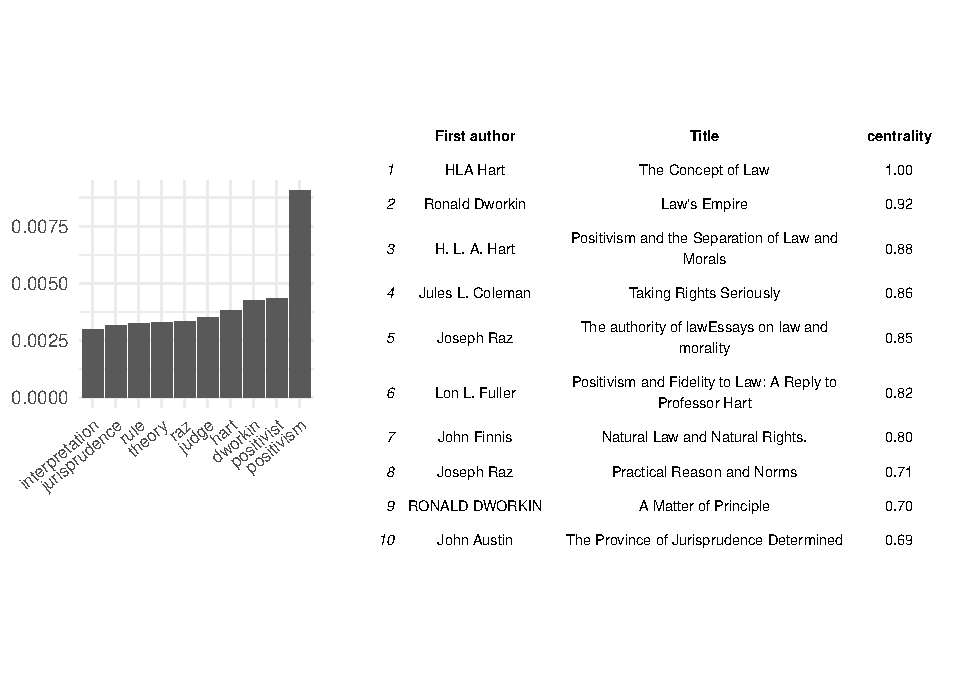
\includegraphics{paper_files/figure-latex/GJ-1} \end{flushright}

\hypertarget{law-and-political-theory-n-83}{%
\subsection{\texorpdfstring{Law and political theory (\emph{N} = 83)}{Law and political theory (N = 83)}}\label{law-and-political-theory-n-83}}

\begin{flushright}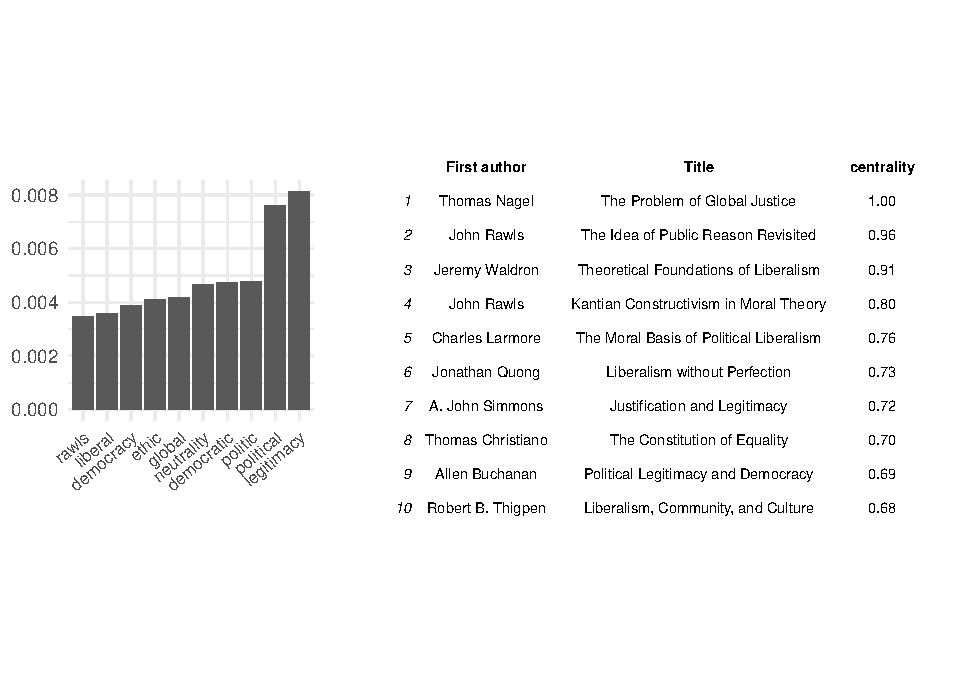
\includegraphics{paper_files/figure-latex/LPT-1} \end{flushright}

\hypertarget{punishment-n-66}{%
\subsection{\texorpdfstring{Punishment (\emph{N} = 66)}{Punishment (N = 66)}}\label{punishment-n-66}}

\begin{flushright}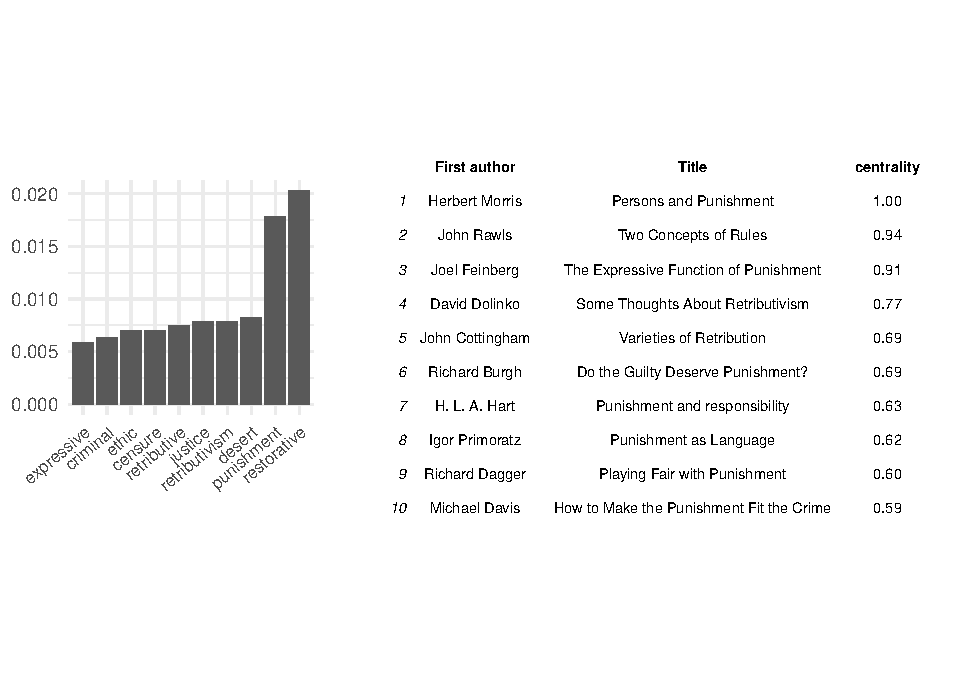
\includegraphics{paper_files/figure-latex/P-1} \end{flushright}

\hypertarget{responsibility-n-60}{%
\subsection{\texorpdfstring{Responsibility (\emph{N} = 60)}{Responsibility (N = 60)}}\label{responsibility-n-60}}

\begin{flushright}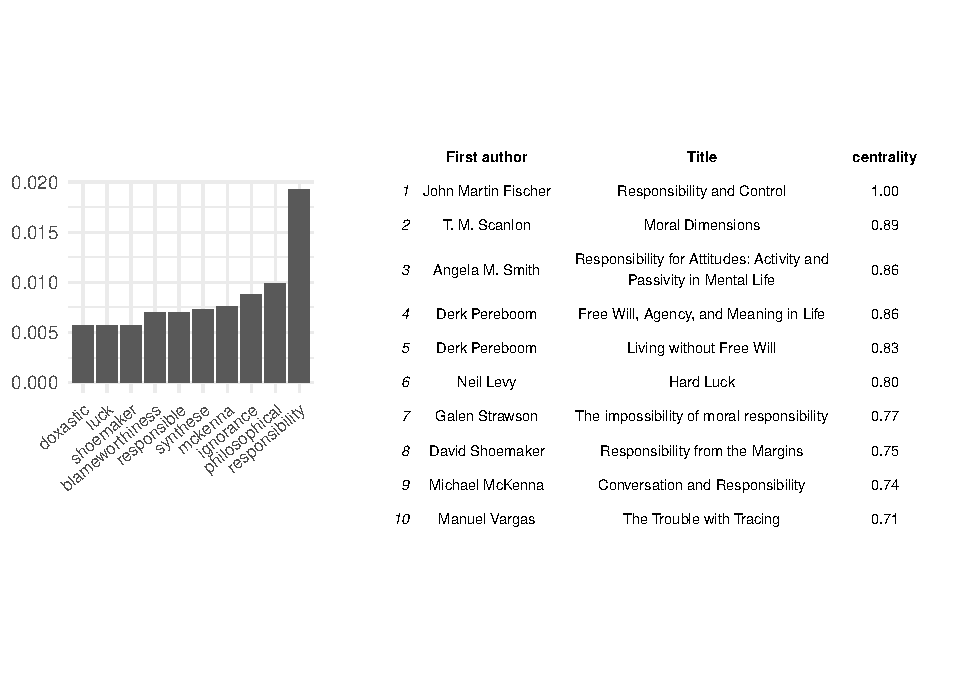
\includegraphics{paper_files/figure-latex/R-1} \end{flushright}

\hypertarget{judicial-review-and-consitutional-rights-n-52}{%
\subsubsection{\texorpdfstring{Judicial review and consitutional rights (\emph{N} = 52)}{Judicial review and consitutional rights (N = 52)}}\label{judicial-review-and-consitutional-rights-n-52}}

\begin{flushright}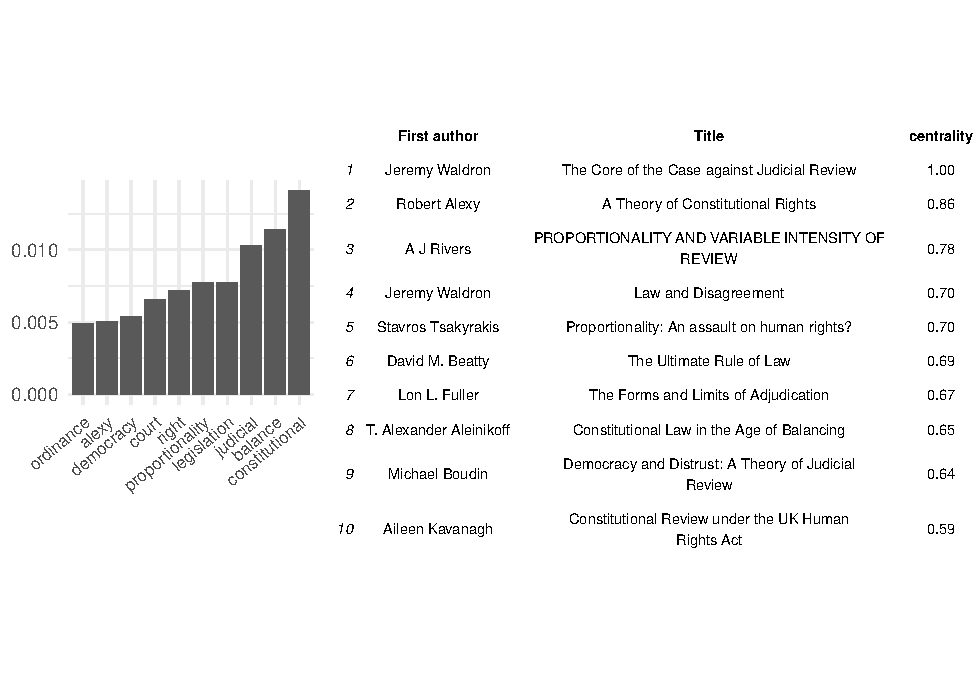
\includegraphics{paper_files/figure-latex/JR-1} \end{flushright}

\hypertarget{torts-causation-n-46}{%
\subsubsection{\texorpdfstring{Torts / causation (\emph{N} = 46)}{Torts / causation (N = 46)}}\label{torts-causation-n-46}}

\begin{flushright}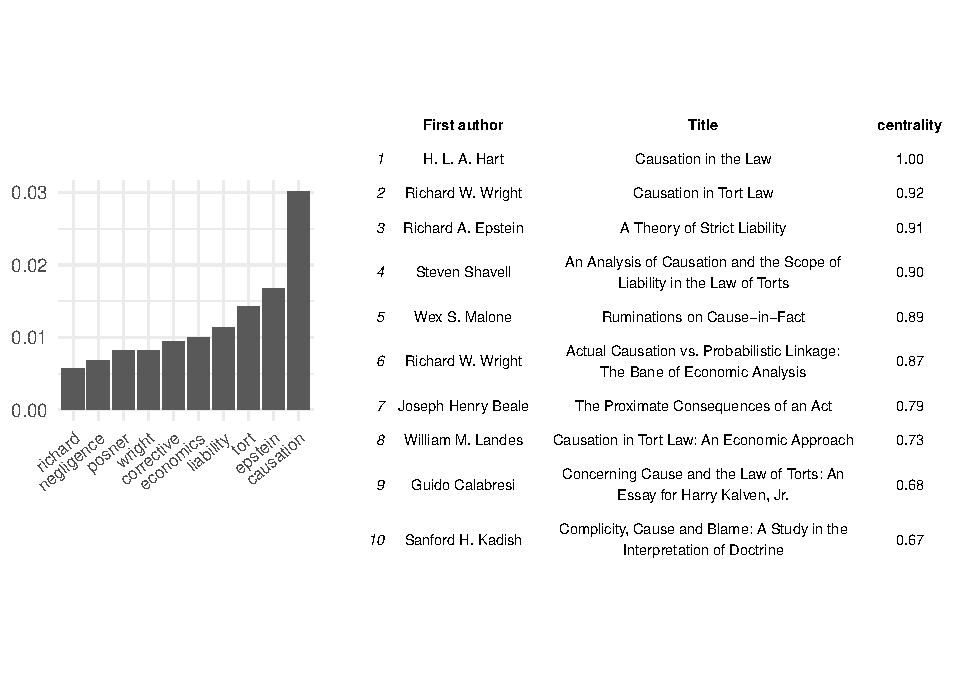
\includegraphics{paper_files/figure-latex/TC-1} \end{flushright}

\hypertarget{theory-of-rights-contracts-n-41}{%
\subsubsection{\texorpdfstring{Theory of rights / Contracts (\emph{N} = 41)}{Theory of rights / Contracts (N = 41)}}\label{theory-of-rights-contracts-n-41}}

\begin{flushright}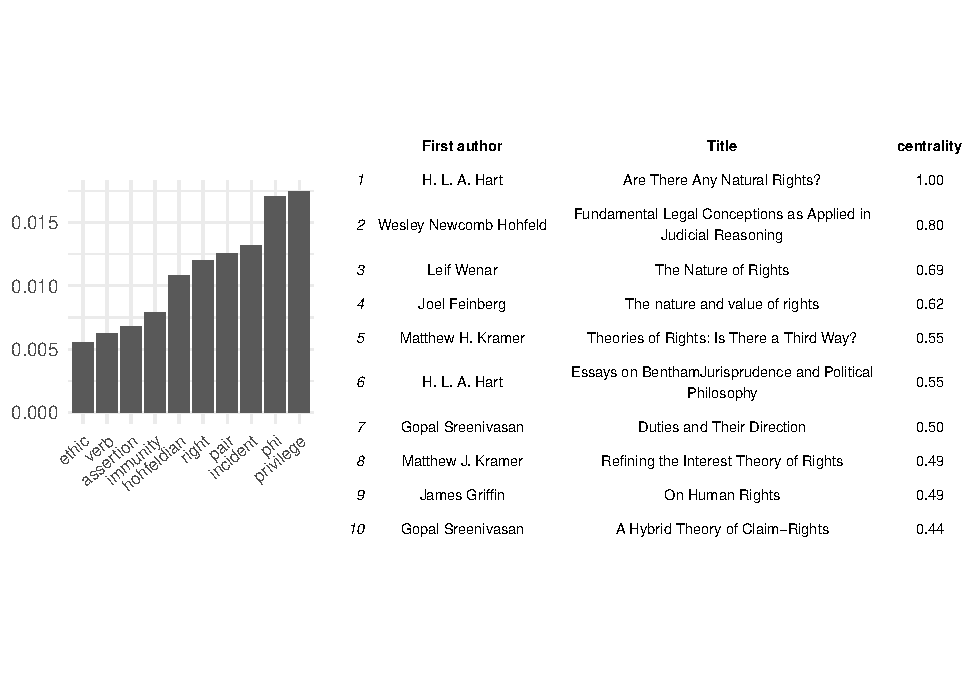
\includegraphics{paper_files/figure-latex/TR-1} \end{flushright}

\end{document}
